\section{An inverse on one fixed annulus}
\label{sec:radial-reference-inverse}

Local spectral gaps do not automatically survive gluing.  A homogeneous
solution can leave one piece, return through its neighbor, and satisfy a
new matching condition.  We must therefore estimate the global matching
problem, not just list the inverses of its pieces.

The frequency decomposition from the preceding section makes this
possible.  At a fixed frequency there are three regions: an inner
collection of well-separated models, one transition cell at each end,
and two deep tails.  The selected height ratios control the matching
angle at the transition cells.  A positive interval just before each
transition prevents its possibly large response from reaching the fixed
interior.  Figure~\ref{fig:frequency-regions} shows this division of labor.
The position of the division changes with frequency; the surface itself
will be chosen once.

\begin{figure}[htbp]
\centering
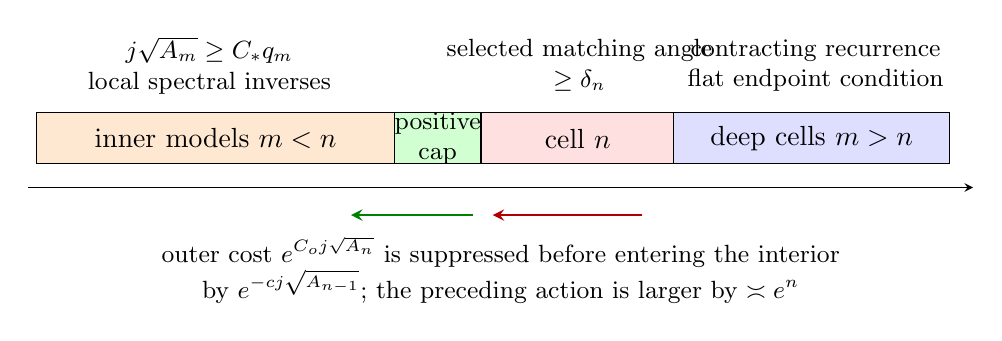
\begin{tikzpicture}[x=1cm,y=1cm,>=stealth]
\draw[->] (0,0)--(12,0);
\draw[fill=orange!18] (.1,.3) rectangle (4.65,.95);
\draw[fill=green!18] (4.65,.3) rectangle (5.75,.95);
\draw[fill=red!12] (5.75,.3) rectangle (8.2,.95);
\draw[fill=blue!13] (8.2,.3) rectangle (11.7,.95);
\node at (2.38,.62) {inner models $m<n$};
\node[align=center,font=\small] at (5.2,.62) {positive\\cap};
\node at (6.98,.62) {cell $n$};
\node at (9.95,.62) {deep cells $m>n$};
\node[align=center,font=\small] at (2.3,1.55)
 {$j\sqrt{A_m}\ge C_*q_m$\\local spectral inverses};
\node[align=center,font=\small] at (7,1.55)
 {selected matching angle\\$\ge\delta_n$};
\node[align=center,font=\small] at (10,1.55)
 {contracting recurrence\\flat endpoint condition};
\draw[->,thick,red!70!black] (7.8,-.35)--(5.9,-.35);
\draw[->,thick,green!50!black] (5.65,-.35)--(4.1,-.35);
\node[align=center,font=\small] at (6,-1.05)
 {outer cost $e^{C_o j\sqrt{A_n}}$ is suppressed before entering the interior\\
 by $e^{-c j\sqrt{A_{n-1}}}$; the preceding action is larger by $\asymp e^n$};
\end{tikzpicture}
\caption{The frequency-dependent decomposition of one end.
The other end is treated simultaneously.  Costs whose output remains
in cell $n$ or farther out can be absorbed by the coefficient weight
there; costs returning to the interior require the preceding positive cap.}
\label{fig:frequency-regions}
\end{figure}

\subsection{Joining the distinguished solution first}
\label{subsec:rad-cone-bump-target-match}

We first finish the actual geometry, keeping its second mode exactly.
On a positive interval put $y=\log r$, $w=re^f$, and prescribe the
logarithmic slope $k=\phi_y/\phi$ of a nonvanishing second-mode solution.
The equation $L_2\phi=0$ is equivalent to
\begin{equation}\label{eq:rad-eq-sp1}
 f_y=\frac{k^2+k_y-4}{4-k},\qquad
 1+f_y=\frac{k^2-k+k_y}{4-k}.
\end{equation}
Thus choosing $k<4$ and $k^2-k+k_y>0$ constructs both the solution and
a positive-curvature connector: integrate $f_y$ and then
$\phi_y=k\phi$.  This is more reliable than interpolating $w$ and
hoping to retain its kernel.

The central slopes tend with all fixed derivatives to $2$ on the left
and $-2$ on the right, by \eqref{eq:rad-eq-sc2}.  Cut sufficiently far
out and interpolate $k$ to the respective constant on a unit $y$
interval.  At either constant the second expression in
\eqref{eq:rad-eq-sp1} equals one, so $C^1$ closeness ensures
$1+f_y\ge3/4$.  Smooth cutoffs match all endpoint germs.
The connector ends in an exact cone, where $k=\pm2$.

On the auxiliary cone of a selected tail, the natural second-mode
solution is $C_+r^2+C_-r^{-2}$.  At the right tail the incoming line
is $r^2$, so the selected nonzero angle implies $C_-\ne0$.
Far toward $r=0$ the natural slope therefore tends to $-2$.
At the left tail the incoming line is $r^{-2}$, and the slope tends
to $2$ toward $r=\infty$.  In both cases the solution is nonzero
sufficiently far along the cone.  The same interpolation of $k$
connects it to an exact cone while retaining $1+f_y\ge3/4$.
Arbitrarily long exact cone segments may be placed between these short
connectors.

A radius change
\begin{equation}\label{eq:rad-eq-ha1}
 \widetilde r=Rr,\qquad \widetilde w(Rr)=Rw(r)
\end{equation}
places each tail at the required radius and preserves $w/r$, $B_j$ and
$\varpi\,dr$.  A subsequent positive height rescaling matches the
additive constant in $f$ without changing homogeneous solutions or
travel angles.  Scaling the tail solution matches its nonzero value.
We obtain one smooth profile $w_*$ and one globally defined, endpoint-flat
second-mode solution $\phi_*$.  We write $w=w_*$ for the rest of this
section.  Only positive pieces have been added, so all
negative travel angles remain those already computed.
What remains to prove is that there is no additional kernel and that
the inverse estimates are uniform.

\subsection{What a positive buffer does to a model inverse}

A useful local fact is that a distant boundary condition produces an
exponentially small change at a cut inside a positive region.  We need
this fact for the operator and for its boundary derivatives, including
the bordered central model.

\begin{lemma}[Cutting inside a positive buffer]\label{lem:fence-compression}
Let $H_0=-\partial_X^2+V$ have a self-adjoint full-model realization.
Allow also a compact symmetric scalar border, supported away from all
cuts.  Suppose the resulting operator $\mathcal H$ is invertible with
$\|\mathcal H^{-1}\|\le B_0$.  At each of at most two cuts $i$, suppose
$V\ge m_i^2$ on the exterior and on an inward interval of length
$(S_i+6)/m_i$.  Suppose $V\le Cm_i^2$ on the cut layer and the inner
cutoff layer, each of width $4/m_i$; any finite exterior wall is at
least $4/m_i$ away.

Let $\alpha_i^{\rm in}$ be the unit-boundary energy of the inward
positive interval with an artificial Dirichlet wall, and
$\alpha_i^{\rm out}$ that of the exterior with its natural condition.
Then $\alpha_i^{\rm in},\alpha_i^{\rm out}\asymp m_i$.
With $D=\operatorname{diag}(\alpha_i^{\rm in}+\alpha_i^{\rm out})$,
the retained Dirichlet operator $\mathcal H_D$, its row-zero Poisson
map $T$, and its outward derivative matrix $\Lambda$ satisfy
\begin{equation}\label{eq:buffer-estimates-new}
 \begin{gathered}
 \|\mathcal H_D^{-1}\|\le B_0+C\sum_i m_i^{-2},\qquad
 \|TD^{-1/2}\|\le C\Bigl(\sum_i m_i^{-2}\Bigr)^{1/2},\\
 D^{-1/2}\bigl(\Lambda-\operatorname{diag}\alpha_i^{\rm in}\bigr)D^{-1/2}
       =O(E),\qquad
 |E_{ik}|\le CB_0m_im_ke^{-S_i-S_k},
 \end{gathered}
\end{equation}
provided $B_0m_i^2e^{-S_i}$ is sufficiently small at every cut.
In particular $\Lambda$ is positive.
\end{lemma}

\begin{proof}
The unit-boundary energy is at least $m_i$ by expanding
$\int|v'\pm m_iv|^2$.  A test function supported within distance
$2/m_i$ gives the matching upper bound.  Join the inward and exterior
unit solutions at the cut; after division by
$\alpha_i^{\rm in}+\alpha_i^{\rm out}$ this is its local point-source
Green function.  Cut it off just before the inner artificial wall,
obtaining $K_i$.  Positive comparison with $-v''+m_i^2v=0$ gives
\[
 \mathcal H(K_i,0)=(\delta_{c_i}+f_i,0),\qquad
 \|K_i\|_2\le Cm_i^{-3/2},\qquad
 \|f_i\|_2\le Cm_i^{1/2}e^{-S_i}.
\]
The scalar coordinate is omitted in the unbordered case; in the bordered
case the cutoff support is disjoint from the border.  The residual is
an ordinary $L^2$ commutator source, not a point source.  Therefore
\[
 \boldsymbol g_i=(K_i,0)-\mathcal H^{-1}(f_i,0)
\]
is the exact Green column at the cut.

Let $\Gamma_{ik}=(g_k)_{\rm field}(c_i)$.  The correction is homogeneous
in the positive buffer at cut $i$ and satisfies the natural exterior
condition.  Propagating it from the inner cutoff layer to the cut costs
a further $e^{-S_i}$; rescaling a layer of width $m_i^{-1}$ converts
its $L^2$ bound to a point bound with factor $Cm_i^{1/2}$.
Consequently
\[
 D^{1/2}\Gamma D^{1/2}=I+E,\qquad
 |E_{ik}|\le CB_0m_im_ke^{-S_i-S_k}.
\]
This also follows directly by applying Green's identity to the two
commutator residuals.  The stated smallness makes this finite matrix
invertible.

Let $\iota$ extend the retained source by zero and $\mathcal R$ restrict
the field, preserving the scalar in both cases.  Subtracting the cut
values gives the exact formulas
\[
 \mathcal H_D^{-1}=\mathcal R\mathcal H^{-1}\iota
                     -\boldsymbol g_I\Gamma^{-1}\boldsymbol g_I^*,
 \qquad T=\boldsymbol g_I\Gamma^{-1}.
\]
There is no hidden kernel: extending a homogeneous Dirichlet field by
zero leaves only cut delta sources, and the invertible cut matrix forces
their coefficients to vanish.  Moreover
\[
 \|\boldsymbol g_iD_{ii}^{1/2}\|
 \le C(m_i^{-1}+B_0m_ie^{-S_i})\le Cm_i^{-1},
\]
which proves the first two bounds.  Interior and exterior derivatives
of a Green column add to its delta coefficient, so
$\Lambda=\Gamma^{-1}-\operatorname{diag}\alpha_i^{\rm out}$.
This gives the final estimate and positivity.  The compact symmetric
border cancels in the same Green identities, so the proof covers it
without an additional boundary term.
\end{proof}

We now translate this estimate to the radial problem.  The exact norm
and flux conversions are
\begin{equation}\label{eq:rad-eq-hn2}
 \|u\|_{L^2(\varpi dr)}^2=12\lambda\int\upsilon^2|\psi|^2\,dX,
 \qquad wu_r=\lambda\sqrt{\mathcal P}
       \left(\psi_X-\frac{\mathcal P_X}{2\mathcal P}\psi\right).
\end{equation}
Using $\sqrt\lambda\psi$ removes the absolute profile amplitude.
For a Morse cell the short and long positive cut regions have,
respectively,
\[
 (m_{X,j},\Delta X,\upsilon)
 \asymp(j\sqrt{A_m},1,A_m),\qquad
 (jA_m^{9/2},A_m^{-4},A_m^5).
\]
Each contains action $c\tau_{m,j}$ with
$\tau_{m,j}=j\sqrt{A_m}$, and $\upsilon/m_{X,j}\le C/j$.
The full-model inverse costs a fixed power of $\mathcal E_m$.
For the central oscillator, far cuts have
$m_{X,j}\asymp j|X|$ and action $cjX^2$; its two-sided weighted
inverse was proved in the preceding section.

The Liouville factor also changes the leading conormal impedance.
At a central cut with outward sign $\epsilon_i$, the exact radial
boundary matrix is
\begin{equation}\label{eq:rad-eq-hn3}
 \Lambda_r=\lambda\operatorname{diag}(\sqrt{\mathcal P_i})
                  \Lambda_X\operatorname{diag}(\sqrt{\mathcal P_i})
          +\lambda a_c\operatorname{diag}(\epsilon_i\mathcal P_i).
\end{equation}
Thus its positive diagonal is
$\kappa_i=\lambda\mathcal P_i(\alpha_i^{\rm in}+\epsilon_i a_c)$,
comparable to $\lambda\mathcal P_i m_{X,j}$ at the chosen far cuts.
For a Morse model it is simply $\lambda\alpha_i^{\rm in}$.
Retaining this gauge term is necessary for exact flux matching.

\subsection{The inner region: retain the full positive interface energy}
\label{subsec:rad-localized-hilbert-assembly}

Fix $j\in\mathcal I_n$.  The finite inner domain consists of the
central model, the earlier cells $m<n$, and their positive connectors.
Its two outer boundaries are the entrances to the selected transition
joins.  Impose zero values there.  At frequency two use the auxiliary
compact symmetric border.  In radial Hilbert notation,
\begin{equation}\label{eq:rad-eq-hn1}
 d\mu=\varpi\,dr,\qquad B_j=-\varpi^{-1}L_j,
 \qquad F=-\varpi^{-1}f,\qquad
 \langle u,F\rangle_{L^2(d\mu)}=-\int\overline u f\,dr.
\end{equation}
For a border column $k=-\varpi^{-1}g_0$, its Hilbert adjoint is
$k^*u=-\ell_0u$; changing the sign of the scalar source row therefore
makes the border symmetric.  This convention will be used in all
intermediate energy identities.

Let $D_h$ be the direct sum of the cut-model Dirichlet inverses and
the exact positive-connector inverses.  On every positive connector,
\begin{equation}\label{eq:rad-eq-hn5}
 Q_j(u)=\int\left(w|u_r|^2+j^2\frac{w'}r|u|^2\right)dr
               \ge cj^2\|u\|_{L^2(d\mu)}^2.
\end{equation}
Here $c=1/6$ on the short joins where $rw'/w\ge2$, and a smaller
fixed positive $c$ covers the cone heads and central connectors.
Its Poisson map $P_C$ and full conormal matrix $\Lambda_C$ consequently
satisfy $\|P_Ca\|\le(C/j)(a^*\Lambda_Ca)^{1/2}$.

A short connector can have a large mixed entry in $\Lambda_C$.
We keep that entry instead of treating it as an error.  At all internal
interfaces set
\begin{equation}\label{eq:rad-eq-hn6}
 S_0=\operatorname{diag}(\kappa_i)+\bigoplus_C\Lambda_C,
 \qquad S=S_0+E_h.
\end{equation}
The positive matrix $S_0$ has blocks of size at most two and dominates
$D_\kappa=\operatorname{diag}(\kappa_i)$.  All errors $E_h$ now
come from crossing positive buffers inside the local models.

To see this uniformly in the number of cells, use a source weight $W$
which is one on the finite middle and has cell size
\begin{equation}\label{eq:rad-eq-hn4}
 W_m=(\mathcal E_m/\mathcal E_N)^{M_0}(H_m/H_N)^{-\gamma}.
\end{equation}
Make it constant across each whole positive gap, with the geometric
mean of the neighboring weights, and vary it inside the model cells.
For $|\gamma|\le1$,
\begin{equation}\label{eq:adjacent-weight-ratio-new}
 |\log(W_{m+1}/W_m)|
 \le Cm^2+CM_0m^{3/2}\log(e+m).
\end{equation}
Thus this interpolation changes cell norms by fixed coefficient powers.
Let $\Omega=\operatorname{diag}(W(c_i))$.  It commutes with $S_0$,
because the two ends of every positive connector have the same weight.

The buffer lemma and \eqref{eq:rad-eq-hn2} give local normalized errors
\begin{equation}\label{eq:rad-eq-hn7}
 \mathcal E_m^{C(M_0)}\langle j\rangle^C e^{-c\tau_{m,j}},\qquad
 C\langle j,X_0\rangle^Ce^{-cjX_0^2},\qquad
 C_N\langle j\rangle^Ce^{-cjL}
\end{equation}
for earlier cells, central cuts and initial cone heads.  The leading
Poisson layer at a model cut has Hilbert norm at most
$(C/j)\sqrt{\kappa_i}|a_i|$, because
$\upsilon/m_{X,j}\le C/j$.  Its remaining part has the first type
of error in \eqref{eq:rad-eq-hn7}.  The assertion of uniform smallness
includes frequencies arbitrarily far above a cell's threshold.  To see
this, put $t=j\sqrt{A_m}\ge C_*q_m$.  Since
$\log\langle j\rangle\le\log(1+t)+Cm^2$, the logarithm of that
local error is bounded, with fixed $a,b,c>0$, by
\begin{equation}\label{eq:inner-uniform-suppression}
 a q_m+b\log(1+t)-ct
 \le a q_m-\tfrac34ct+C_b
 \le-\tfrac12ct+C_b
 \quad\text{if }C_*\ge4a/c.
\end{equation}
Here $m^2=o(q_m)$ was included in $a$, and the middle inequality uses
$b\log(1+t)\le ct/4+C_b$.  Increasing $N$ now makes the original error
smaller than any prescribed positive tolerance, simultaneously for all $m<n$
and all such $j$.  Thus we choose $M_0$ for source conversion, then
$C_*$, then $N$, and finally the central cuts and the fixed head
lengths.  Their errors in \eqref{eq:rad-eq-hn7} have the same
polynomial-versus-exponential comparison, on the finitely many central
pieces.

Let $T_h$ be the homogeneous interpolation of common interface values,
with zero scalar row.  The resulting two estimates are
\begin{equation}\label{eq:rad-eq-hn8}
 \begin{gathered}
 \|S_0^{-1/2}\Omega^\epsilon E_h\Omega^{-\epsilon}S_0^{-1/2}\|<1/2,\\
 \|W^\epsilon T_h\Omega^{-\epsilon}S_0^{-1/2}\|\le C/j,
 \qquad \epsilon=\pm1.
 \end{gathered}
\end{equation}
For the first, normalize each model error by its two adjacent
$\kappa_i^{1/2}$.  Each interface belongs to at most two such blocks,
so their sum has operator norm at most twice the largest local norm.
Then use $\|S_0^{-1/2}D_\kappa^{1/2}\|\le1$ on both sides.
For the second, sum the squared local Poisson norms over disjoint model
interiors and over the positive connectors, whose overlap is bounded.
This proves both estimates independently of the number of cells.

The outgoing interface flux of a zero-boundary source solution is
$-T_h^*F$.  Matching values and fluxes therefore gives the exact inverse
\begin{equation}\label{eq:rad-eq-hn9}
 G_h=D_h+T_hS^{-1}T_h^*.
\end{equation}
The two signs of the weight in \eqref{eq:rad-eq-hn8} control the second
term by duality.  Local Dirichlet costs are coefficient powers, so,
for a sufficiently large fixed $M_1$,
\begin{equation}\label{eq:inner-inverse-estimates-new}
 \|W_1G_hW^{-1}\|\le C,\qquad
 \|W^{\pm1}G_hW^{\mp1}\|\le\mathcal E_n^C,
 \qquad W_1=W(\mathcal E/\mathcal E_N)^{-M_1}.
\end{equation}
The first estimate is localized and will handle ordinary inner sources.
Its net output coefficient exponent is $M_0-M_1$; at the end we rename
$M_1-M_0>0$ as the output exponent in
Proposition~\ref{prop:rad-fixed-theorem}.
The coarser second estimate is used only on boundary residuals which
already contain an exponentially small factor.  Invertibility of the
Dirichlet blocks and of $S$ proves both inverse identities in
\eqref{eq:rad-eq-hn9}; its symmetry is the corresponding Green identity.

\subsection{The transition region and an outer inverse without division by height}

The outer core begins at a selected join, contains cell $n$, and ends
where the deep tail starts.  The preceding large positive cap belongs
to the inner domain.  On the right the deep entrance is a mass entrance;
on the left it is the initial resistance entrance described earlier.
Let $r_o$ increase outward, use positive measure $dr_o$, and choose
$\lambda>0$ with $e^{-Cn^2}\le\lambda/\lambda_n\le e^{Cn^2}$.
In the state $(u,z)$, $z=wu_{r_o}/\lambda$, the core has the bounds
\begin{equation}\label{eq:transition-inputs-new}
 \begin{gathered}
 \|T\|+\|T^{-1}\|\le\mathcal K_n:=e^{Cn^2+C_o\tau_{n,j}},
 \qquad \int_{\rm core}\varpi\,dr_o\le\lambda e^{Cn^2},\\
 \|P_d\|_{L^2(d\mu)}\le\sqrt\lambda e^{Cn^2},
 \qquad \|B_{d,D}^{-1}\|\le Cj^{-4}.
 \end{gathered}
\end{equation}
Here $P_d$ is the deep natural solution with entrance value one.

For clarity, these four estimates follow from different parts of the
construction.  The last is \eqref{eq:rad-eq-rm20}.
The core mass is $12\lambda_n\int(v/r)^2dX$, plus the negligible
joining masses, so it has the stated size by
\eqref{eq:rad-eq-rm6}.  The weighted node contraction
\eqref{eq:rad-eq-dg4} bounds the squared norm of $P_d$ by the first
deep mass.  If an initial resistance edge comes first, its next mass
height is at most $C/(\Lambda\mu R_0)$ and the edge mass is small;
the same bound follows.
For the transfer estimate, on a positive piece the off-diagonal
coefficients in $(u,z)$ are $\lambda/w$ and $j^2w_r/(\lambda r)$.
Balancing their integrals bounds the transfer in either direction by
\[
 e^{Cn^2}\exp\!\left(2j\sqrt{\left(\int dr_o/w\right)
                                  \left(\int w_r\,dr_o/r\right)}\right).
\]
The product inside the square root is $O(A_n)$ on either positive cap
and smaller on the short join.  On the negative component use
$u_{XX}+j^2\rho u=0$ and the energy
$E=|u_X|^2+(1+j^2\rho)|u|^2$.
It satisfies
$|E_X|\le[1+j^2|\rho_X|/(1+j^2\rho)]E$.
The interval has length $O(n^2)$ and $\rho$ has one peak, so the
integrated second term is at most $2\log(1+j^2\max\rho)$.
Converting the flux back to $(u,z)$ costs only $e^{Cn^2}$.
Together these estimates prove \eqref{eq:transition-inputs-new}.

The natural outer solution may vanish at the entrance.  A logarithmic
slope there is therefore the wrong variable.  Normalize its full state:
\begin{equation}\label{eq:rad-eq-tm1}
 v=(V(r_{o,-}),f_V(r_{o,-})/\lambda),\qquad |v|=1,
 \qquad f_u=wu_{r_o},\qquad v^\perp=(-v_2,v_1).
\end{equation}
Let $U$ have entrance state $v^\perp$.  For $\mathscr H_j=-L_j$,
the kernel
\[
 K_o(r_o,t_o)=\lambda^{-1}U(\min(r_o,t_o))V(\max(r_o,t_o))
\]
has the natural endpoint condition and the complementary Robin condition
$v\cdot(u,f_u/\lambda)=0$ at the entrance.  Its normalization is exact:
$w(UV_{r_o}-U_{r_o}V)=-\lambda$.
Thus
\begin{equation}\label{eq:outer-robin-new}
 R_oF=\int K_o(r_o,t_o)F(t_o)\,d\mu(t_o),\qquad
 G_of=-\int K_o(r_o,t_o)f(t_o)\,dt_o
\end{equation}
are respectively the Hilbert inverse of $B_j$ and the original-source
inverse of $L_j$.  No entrance height has been divided out.
Green's identity gives the remaining boundary equation
\begin{equation}\label{eq:rad-eq-tm2}
 v^\perp\cdot(u,f_u/\lambda)
       =\lambda^{-1}\int V\varpi F\,dr_o,
 \qquad \|V\|_{L^2(d\mu)}\le\sqrt\lambda\mathcal E_n^C\mathcal K_n.
\end{equation}
The natural endpoint term is zero by the deep-tail construction.

The factor $\lambda^{-1}$ in the kernel causes no amplitude loss.
On the core it is canceled by the mass bound in
\eqref{eq:transition-inputs-new}.  On the deep region exact kernel
restriction gives
\[
 (R_o)_{d,d}=B_{d,D}^{-1}+P_dK_o(r_{o,+},r_{o,+})P_d^*,
 \qquad |K_o(r_{o,+},r_{o,+})|
        \le\lambda^{-1}\mathcal E_n^C\mathcal K_n^2.
\]
The two Poisson norms cancel it there, and the cross blocks have one
Poisson factor each.  Consequently
\begin{equation}\label{eq:rad-eq-tm3}
 \|R_o\|\le\mathcal E_n^C\mathcal K_n^2.
\end{equation}
The localized deep kernel \eqref{eq:rad-eq-dj5} and the outward
homogeneous quotient \eqref{eq:rad-eq-rm17} give more precisely
\begin{equation}\label{eq:rad-eq-tm4}
 \|\vartheta_kR_o\vartheta_m\|
 \le\mathcal E_k^C\mathcal E_m^C\mathcal K_n^2 e^{-|S_k-S_m|},
 \qquad k,m\ge n-O(1).
\end{equation}
A product of two outward quotient factors is bounded by the same
exponential, since both indices lie beyond the entrance.
Converting the source and target to $L^2(dr_o)$ adds
$\varpi^{-1/2}$ on each of their cells, bounded by coefficient powers.
Hence \eqref{eq:rad-eq-tm4} also holds for $G_o$ in ordinary source
units.  These observations justify both inverse identities and
reciprocity directly from the kernel.

\subsection{The two boundary values which remain to be matched}
\label{subsec:terminal-matching}

At each truncation boundary use the scale
$\lambda_i=j^2W_{{\rm in},i}/r_{{\rm in},i}$.
Its ratio to the transition-cell height is between $e^{-Cn^2}$ and
$e^{Cn^2}$, so the preceding outer estimates apply.
Let $\kappa_i$ be the impedance of the artificial incoming positive
block used for height selection and put
$d_i=\kappa_i/\lambda_i$, $D_0=\operatorname{diag}(d_i)$.
The incoming estimate gives $0<d_i\le1/2$; in the first band $d_i=1/j$.
Use normalized boundary coordinates
$x_i=\sqrt{\lambda_i}u_i$, $z_i=f_{u,i}/\sqrt{\lambda_i}$.

Let $\mathcal B_h$ denote the inner Hilbert operator, including its
symmetric scalar border, and let $\mathcal Q_h$ be its quadratic form.
We need to know how much the true inner derivative matrix differs
from this artificial incoming one.  Take its positive-block Poisson
function of boundary height $\lambda_i^{-1/2}$, cut it off near the
inner end of that block, and extend by zero.  Call the resulting field
$\mathcal L_i$, and its ordinary Hilbert residual
$\mathcal F_i=\mathcal B_h\mathcal L_i$, including zero scalar row.
Allocate separate fixed fractions of the preceding cap to this cutoff
and to the earlier model's buffer.  Positive comparison and the
commutator
\[
 \mathscr H_j(\chi u)-\chi\mathscr H_ju
       =-2w\chi'u'-(w\chi')'u
\]
then give
\begin{equation}\label{eq:rad-eq-tm6}
 \begin{gathered}
 \|W^{\pm1}\mathcal L_i\omega_i^{\mp1}\|
       \le C\sqrt{d_i}/j,\qquad
 \|W^{\pm1}\mathcal F_i\omega_i^{\mp1}\|
       \le\sqrt{d_i}\mathcal E_n^Ce^{-S_{b,i}},\\
 S_{b,i}=c\tau_{n-1,j}\quad\text{or, in the first band, }cjL.
 \end{gathered}
\end{equation}
Here $\omega_i$ is the constant weight on this positive gap.
The first bound uses the energy $\kappa_i/\lambda_i=d_i$ and
\eqref{eq:rad-eq-hn5}; the second uses the extra attenuation on the
cutoff layer.  The two lifts have disjoint supports, and their energy
matrix is diagonal with entries
$d_i(1+O(\mathcal E_n^Ce^{-2S_{b,i}}))$.

The exact homogeneous Poisson map is
$P_h=\mathcal L-G_h\mathcal F$.
Completing the quadratic form gives the true normalized derivative
matrix
\begin{equation}\label{eq:rad-eq-tm7}
 D_b=\mathcal Q_h(\mathcal L,\mathcal L)-\mathcal F^*G_h\mathcal F
       =D_0+E_b,
 \qquad |(E_b)_{ik}|\le
     \mathcal E_n^C\sqrt{d_id_k}e^{-S_{b,i}-S_{b,k}}.
\end{equation}
The two cross terms cancel one correction term because
$\mathcal B_hG_h\mathcal F=\mathcal F$ and the correction has zero
boundary values.  This identity is also why the error has \emph{two}
attenuation factors.  The scalar border is symmetric and every lift
has row zero, so there is no missing scalar term.

Use the outer normalized states \eqref{eq:rad-eq-tm1} with these
$\lambda_i$.  Let $A=\operatorname{diag}(v_{1,i})$,
$B=\operatorname{diag}(v_{2,i})$, and let $\mathcal V$ consist of
the two outer columns $V_i/\sqrt{\lambda_i}$.
The inner source flux is $-P_h^*F_h$, while
\eqref{eq:rad-eq-tm2} supplies the outer equation.  Thus the complete
matching problem is just
\begin{equation}\label{eq:rad-eq-tm8}
 z=D_bx-P_h^*F_h,\qquad -Bx+Az=\mathcal V^*F_o,\qquad
 Kx=\mathcal V^*F_o+AP_h^*F_h,\quad K=A(D_0+E_b)-B.
\end{equation}

The angle selected in the preceding section is exactly what is needed
to invert the diagonal part of $K$.  Its state is
$(u,-u\pm f_u/\lambda_i)$; the change to $(u,f_u/\lambda_i)$
has a fixed condition number.  Transport across the nearly identity
join preserves the angle lower bound up to a fixed factor.  Hence
\begin{equation}\label{eq:rad-eq-tm9}
 |v_{1,i}d_i-v_{2,i}|
 =\sqrt{1+d_i^2}\,|\sin\angle(v_i,(1,d_i))|
 \ge c\delta_n.
\end{equation}
This argument remains valid when $v_{1,i}=0$.
Any later dependence of the central connectors on the selected tails
is confined to $E_b$; the artificial incoming direction itself was
fixed before the height parameter was varied.

Two estimates now decide the choice of scales:
\begin{equation}\label{eq:rad-eq-tm10}
 \delta_n^{-1}\|E_b\|<c/4,\qquad
 \mathcal E_n^C\delta_n^{-1}
     e^{C_o\tau_{n,j}-c\tau_{n-1,j}}<1/4.
\end{equation}
The first makes $K$ invertible.  The second controls responses which
return to the fixed interior.  They are compatible because
\[
 \tau_{n-1,j}/\tau_{n,j}\asymp e^n,\qquad
 \tau_{n-1,j}\ge C_*q_{n-1},\qquad
 q_n/q_{n-1}\to1,\qquad n^2/q_{n-1}\to0.
\]
Choose $C_*$ after the fixed coefficient exponent, then $N$ large.
The first relation absorbs $C_o\tau_{n,j}$ into a quarter of the
preceding action, and the other relations absorb $Cq_n+n^2+|\log c_0|$
into another quarter.  The first estimate has two such attenuations
by \eqref{eq:rad-eq-tm7}.  At the finite initial band choose the fixed
cone-head length $L$ large enough instead.  Therefore
$\|K^{-1}\|\le C\delta_n^{-1}$ uniformly in the band and frequency.

\subsection{The global estimate and the order of choices}

Set $K_1=A+BD_b$.  Solving \eqref{eq:rad-eq-tm8} and reconstructing
the outer homogeneous coefficient gives the exact matched inverse
\begin{equation}\label{eq:rad-eq-tm11}
 G=\begin{pmatrix}G_h&0\\0&R_o\end{pmatrix}
  +\begin{pmatrix}P_h&0\\0&\mathcal V\end{pmatrix}
   \begin{pmatrix}
       K^{-1}A&K^{-1}\\K^{-T}&K_1K^{-1}
   \end{pmatrix}
   \begin{pmatrix}P_h^*&0\\0&\mathcal V^*\end{pmatrix}.
\end{equation}
For example, the outer coefficient is
$K_1x-BP_h^*F_h$.  Since $D_b=D_b^T$, $A,B$ commute and
$A^2+B^2=I$, direct multiplication gives
\[
 KA=AK^T,\qquad K^TK_1=K_1^TK,\qquad
 K_1K^{-1}A-B=K^{-T}.
\]
These identities prove both the formula and the symmetry of its middle
matrix, whose norm is $O(\delta_n^{-1})$.
We choose equal boundary weights at the two ends by using their common
band index.  A bounded index shift changes their ratio only by a
coefficient power and has the same estimates.

There are two ways to pay for a boundary correction.  We give the
weighted estimate explicitly for each, because this is where local
inverse bounds become an estimate on the whole annulus.

\paragraph{An outer block and its coefficient weights.}
First consider terms involving only $R_o$, $\mathcal V$ and the leading
lifts $\mathcal L$.  Their source and output indices are at least
$n-O(1)$.  Combining \eqref{eq:rad-eq-tm4} with
$\|K^{-1}\|\le C\delta_n^{-1}$ gives, after increasing fixed constants,
\[
 \|\vartheta_kG_{\rm out}\vartheta_m\|
 \le C\exp\{a(q_k+q_m)+d q_n-|S_k-S_m|\}.
\]
Here $d$ includes the finite-core cost: indeed
$\delta_n^{-1}e^{C_o\tau_{n,j}}
 \le c_0^{-1}\exp(n^2+C_oC_*q_n)$.
Since the output is outer, $q_n\le c_1q_k+C_1$; write $d_1=dc_1$.
For $\Delta S=S_k-S_m$, conjugation by the source and output weights
therefore gives the following exact exponent bound:
\begin{equation}\label{eq:outer-weighted-block}
 \begin{aligned}
 \log\|\vartheta_kW_1G_{\rm out}W^{-1}\vartheta_m\|
 &\le C-(M_1-2a-d_1)q_k\\
 &\quad +(a-M_0)(q_m-q_k)-|\Delta S|+\gamma\Delta S.
 \end{aligned}
\end{equation}
Fixed neighboring-index and source-measure changes have been included
in $a,d_1,C$.  Choose $M_1>\max(M_0,2a+d_1)$, after $C_*$.
For any $0<\gamma\le\gamma_+<1$, use
\[
 |q_m-q_k|\le\varepsilon|S_m-S_k|+C_\varepsilon,
 \qquad
 \varepsilon=\frac{1-\gamma_+}{2(1+|a-M_0|)}.
\]
Then \eqref{eq:outer-weighted-block} is at most
$C_\gamma-\tfrac12(1-\gamma_+)|S_k-S_m|$.
This is a summable block kernel in both indices.  On either tail, with
$s_0=\inf_{m\ge N}(S_{m+1}-S_m)>0$ and
$\eta=\tfrac12(1-\gamma_+)$, we have
\[
 \sup_k\sum_m e^{-\eta|S_k-S_m|}
 \le1+\frac{2}{e^{\eta s_0}-1}.
\]
The same estimate holds with $k,m$ reversed.  The two endpoint copies
and the bounded overlap of the localizers change it only by a fixed
factor.  The block Schur estimate proves the outer contribution to the
desired operator bound.
Notice that increasing the output exponent works precisely because
$k$ is near or beyond the transition index; it gives no such estimate
at a fixed interior output.

\paragraph{A boundary block returning to the interior.}
The upper-right block of \eqref{eq:rad-eq-tm11} is
$P_hK^{-1}\mathcal V^*$.  Substituting
$P_h=\mathcal L-G_h\mathcal F$, its part which can reach the fixed
interior is
\[
 C_{ho}=-(G_h\mathcal F)K^{-1}\mathcal V^*.
\]
Let $\Omega$ be the common boundary weight, and use $W_h,W_o$ for
the restrictions of $W$.  The preceding estimates supply
\begin{equation}\label{eq:boundary-column-weights}
 \begin{gathered}
 \|W_hG_h\mathcal F\Omega^{-1}\|
       \le\mathcal E_n^{C_1}e^{-c\tau_{n-1,j}},\\
 \|\Omega K^{-1}\Omega^{-1}\|\le C\delta_n^{-1},\\
 \|\Omega\mathcal V^*W_o^{-1}\|
       =\|W_o^{-1}\mathcal V\Omega\|
       \le C_\gamma\mathcal E_n^{C_2}e^{C_o\tau_{n,j}}.
 \end{gathered}
\end{equation}
The first is \eqref{eq:inner-inverse-estimates-new} applied to the
residual bound \eqref{eq:rad-eq-tm6}; $d_i\le1/2$ absorbs its two
boundary factors.  The middle bound uses equal weights at the two
ends.  For the last bound, the localized column has decay
$\mathcal E_n^C\mathcal E_k^C e^{C_o\tau_{n,j}}e^{-(S_k-S_n)}$.
After either sign of the weight, its extra exponent is
$(C\pm M_0)(q_k-q_n)-(1\mp\gamma)(S_k-S_n)$.
The same slow-variation inequality used above makes its squared sum
finite, leaving a fixed coefficient power at $n$ and a constant
$C_\gamma$.  This proves the displayed adjoint estimate as well as its
reciprocal-weight version.

Multiplying the three factors in \eqref{eq:boundary-column-weights}
now exhibits the two competing costs in one operator estimate:
\begin{equation}\label{eq:one-boundary-cross-block}
 \begin{aligned}
 \|W_hC_{ho}W_o^{-1}\|
 &\le C_\gamma\mathcal E_n^C\delta_n^{-1}
             e^{C_o\tau_{n,j}-c\tau_{n-1,j}}\\
 &\le C_\gamma e^{-c\tau_{n-1,j}/2}\le C_\gamma.
 \end{aligned}
\end{equation}
The second line is the explicit exponent comparison proving
\eqref{eq:rad-eq-tm10}; enlarge the constants there before choosing
$C_*,N$.  For the initial finite band replace the preceding action by
$cjL$.  On the tails $\mathcal E/\mathcal E_N\ge1$, while its smooth extension
has a positive minimum on the fixed middle.  Thus $W_1\le C_{\rm mid}W$
with a fixed constant, which gives the required output-weight bound.
The transpose block uses the opposite sign of the weight in
\eqref{eq:boundary-column-weights}.  Terms with two residual columns
have two preceding attenuations; terms with one residual and one leading
lift have the same estimate.  Thus every correction in
\eqref{eq:rad-eq-tm11} is covered, while the direct inner term is
already bounded by \eqref{eq:inner-inverse-estimates-new}.
We conclude
\begin{equation}\label{eq:global-reference-bound-new}
 \|W_1GW^{-1}\|\le C
\end{equation}
at angular order zero, with the original source-density conversions
included by the coefficient powers already used above.

\begin{lemma}[One geometry for all flat exponents]
\label{lem:radial-uniform-exponents}
The profile, height choices, central cuts and cone-head lengths can be
chosen once so that \eqref{eq:global-reference-bound-new} holds for every
compact range $[\gamma_-,\gamma_+]\Subset(0,1)$.  Only the norm
constants and coefficient exponents may depend on that range.
\end{lemma}
\begin{proof}
Every finite matching choice uses only adjacent weight ratios.
Estimate~\eqref{eq:adjacent-weight-ratio-new} is uniform for
$|\gamma|\le1$.  Fix a source exponent $M_0$ which absorbs the
original-source conversion, then choose $C_*,N$, the central cuts
and head lengths using that uniform bound.  In particular, the
invertibility of $S$ and $K$ is independent of a compact range of
flat exponents.

After this geometry is fixed, the only new issue is the infinite
summation of the deep kernel.  Conjugation by $H^{-\gamma}$ changes
its exponential factor to
\[
 e^{-|S_k-S_m|+\gamma(S_k-S_m)}
      \le e^{-(1-|\gamma|)|S_k-S_m|}.
\]
Its row and column sums are finite when $|\gamma|\le\gamma_+<1$.
Coefficient factors are absorbed using
\[
 |q_k-q_m|\le\varepsilon|S_k-S_m|+C_\varepsilon,
\]
which follows from $q'(x)/S'(x)\to0$.
Choose $\varepsilon$ after $\gamma_+$; this changes the summation
constant and output exponent, not the geometry.  The boundary terms
which enter the interior have already acquired the attenuation in
\eqref{eq:rad-eq-tm10}.  Compact-range summation constants multiply an
existing bound and do not enter the finite matrix inversions.
Thus no later choice of endpoint exponent changes the profile.
\end{proof}

The same estimates with one radial derivative use the local equation
rather than differentiating a spectral decomposition.  On a slightly
enlarged cell,
\begin{equation}\label{eq:rad-eq-rm39}
 \begin{aligned}
 \|u_r\|_2&\le\mathcal E_m^C\bigl(\|f\|_2+(1+j)\|u\|_2\bigr),\\
 \|u_{rr}\|_2&\le\mathcal E_m^C\bigl(\|f\|_2+(1+j^2)\|u\|_2\bigr).
 \end{aligned}
\end{equation}
To derive the first, use interval interpolation
$\|u_r\|_2^2\le C\|u\|_2(\|u_{rr}\|_2+\|u\|_2)$ and substitute
$wu_{rr}=f-w'u_r+j^2w'u/r$; absorb the resulting
$C\|u\|_2\|u_r\|_2$ by Young's inequality.  Substitution back gives
the second.  Rescaling and the reciprocal profile cost coefficient
powers.  A cutoff on the enlarged interval supplies the displayed
local version without imposing a boundary condition.  At mode two
replace $f$ by $f-\nu g_0$, a compact contribution already controlled
by its scalar norm.
Thus one normal derivative uses at most one extra angular derivative.
On an outer transition region any fixed $j$ power is itself bounded
by a coefficient power, since $j<\mathcal H_n$.

\subsection{The realization, the zero mode and the final border}

We now identify the common domain and complete the statement of
Proposition~\ref{prop:rad-fixed-theorem}.

\begin{definition}[The weighted graph domain]\label{def:radial-graph-domain}
Let $\mathcal Y_\gamma^{\rm rad}$ be the source space
\eqref{eq:rad-eq-source-norm} at order zero with
$\int\langle f\rangle\,dr=0$, including its scalar row.
Let $\mathcal X_\gamma^{\rm rad}$ consist of $(u,\nu)$ with
$u=a_L\chi_L+v$ and squared norm
\[
 |a_L|^2+|\nu|^2+
 \sum_m\mathcal E_m^{-2M_1}H_m^{-2\gamma}
               \|\vartheta_mv\|_{L^2(dr\,d\theta)}^2.
\]
The angular measure is normalized.  Define
\[
 \begin{aligned}
 \mathcal D_\gamma^{\rm rad}
 &=\{(u,\nu)\in\mathcal X_\gamma^{\rm rad}:
          \mathbb L_w(u,\nu)\in\mathcal Y_\gamma^{\rm rad}\},\\
 \|U\|_{\mathcal D_\gamma^{\rm rad}}
   &=\|U\|_{\mathcal X_\gamma^{\rm rad}}
        +\|\mathbb L_wU\|_{\mathcal Y_\gamma^{\rm rad}}.
 \end{aligned}
\]
The differential expression is interpreted distributionally.  This
definition applies first to the auxiliary border and then to the final
one below.
\end{definition}

The zero mode has not entered the spectral construction.  It is solved
exactly by two primitives.  For $\int f_0\,dr=0$, set
\begin{equation}\label{eq:rad-eq-rm49}
 p_0(r)=\int_{r_-}^r f_0(t)\,dt=-\int_r^{r_+}f_0(t)\,dt,\qquad
 u_0(r)=-\int_r^{r_+}\frac{p_0(t)}{w(t)}\,dt.
\end{equation}
Then $(wu_0')'=f_0$, the right height is zero, and the left height is
an allowed constant.  Summing the cells beyond $n$ gives
$|p_0|\le\mathcal E_n^CH_n^\gamma\|f_0\|_{Y_{\gamma,0}}$.
Division by $w$ and one integration cost only coefficient powers, so
the primitive converges and has the required endpoint estimate after
subtracting $a_L\chi_L$.  The coefficient $a_L$ is a bounded source
functional.  A nonzero homogeneous flux would produce
$\int dr/w$, excluded by its growth; a constant is excluded by the
right normalization.  The zero channel is therefore unique.

\begin{lemma}[The two inverse identities and the graph closure]
\label{lem:rad-green-completion}
The matched nonzero-mode inverse \eqref{eq:rad-eq-tm11} and the zero-mode
primitive \eqref{eq:rad-eq-rm49} define
$\mathbb G_w:\mathcal Y_\gamma^{\rm rad}\to\mathcal D_\gamma^{\rm rad}$.
They satisfy
\begin{equation}\label{eq:rad-reference-piecewise-left-identity}
 \mathbb L_w\mathbb G_w=I,\qquad
 \mathbb G_w\mathbb L_w=I.
\end{equation}
The graph domain is the graph closure of smooth admissible fields.
The Green identities have the ordinary $dr$ source pairing, including
the chosen scalar border.
\end{lemma}
\begin{proof}
On compact smooth finite-frequency sources, all blocks were constructed
as genuine inverses, and their values and conormals match exactly.
Their bounded estimates therefore give the first identity by density.

For uniqueness on the maximal graph domain, subtract this constructed
solution from any other one.  At each fixed nonzero frequency the
homogeneous difference is locally $H^2$, because $w>0$ in the
interior.  Its value and conormal agree at every finite interface.
The endpoint weights put it in the natural Hilbert space, since
$\gamma S_m-Cq_m\to+\infty$ for every fixed $C$.
The deep lemma therefore puts it on the unique natural line at each
end.  Its two remaining boundary values vanish by the invertible
matrix $K$; the inner and outer inverses then make the whole difference
zero.  The zero mode is unique by the primitive calculation.
This proves the second identity without imposing additional traces
at the flat endpoints.

Distributional convergence of a graph-convergent sequence identifies
its limiting image, so the maximal graph domain is closed.
Smooth compact finite-frequency sources are dense in the compatible
source space: truncate and mollify, then restore the integral using
a fixed compact bump of integral one.  Their images are smooth
admissible fields, flat in the nonzero modes outside the support of the
source.  The output bound and the first identity imply convergence in
graph norm; the second identity shows that every graph-domain field
is reached this way.  Finally, the local Green identities and the
symmetric middle matrix in \eqref{eq:rad-eq-tm11} give the stated
reciprocity, with the source conversion in \eqref{eq:rad-eq-hn1}.
\end{proof}

The explicitly joined second-mode solution spans the unbordered kernel:
otherwise its bordered inverse could not be injective.  Its auxiliary
row is nonzero, and we normalize that row to one.
Choose a nonzero $\chi\ge0$ supported on a right positive connector
where $\phi_*'/\phi_*<0$.  Integration by parts gives
\begin{equation}\label{eq:ct-positive-shape}
 a_*:=\int\phi_*L'_{2,w}[w\chi]\phi_*\,dr
 =\int w\chi\left(-\phi_*'^2+\frac{8\phi_*\phi_*'}r
                              -\frac{4\phi_*^2}{r^2}\right)dr<0.
\end{equation}
Put
\begin{equation}\label{eq:rad-eq-ct9}
 \chi_*=\chi/a_*,\qquad
 g_*=L'_{2,w}[w\chi_*]\phi_*,\qquad
 \ell_*u=\int g_*u_2\,dr.
\end{equation}
Then $\int g_*\phi_*\,dr=1$, or equivalently $\ell_*(\phi_*e_2)=1$.
For a source $f_2$, its scalar obstruction is
$\nu=\int\phi_*f_2\,dr$.
Solve the compatible source $f_2-\nu g_*$ with the auxiliary border,
and add a multiple of $\phi_*$ to impose the new row.  This finite-rank
change is bounded in all the established endpoint spaces and preserves
both inverse identities and the graph closure.  From now on
$\mathbb L_{w_*},\mathbb G_{w_*}$ refer to this final border.
All claims in Proposition~\ref{prop:rad-fixed-theorem} now follow.

\paragraph{The interface with the nonlinear argument.}
The result just proved is an angular-order-zero inverse with no angular
loss, together with its first-normal estimate and its maximal graph
domain.  These are the inputs to the subsequent two-weight argument.
For higher normal derivatives, the equation recursively replaces two
normal derivatives by at most two angular derivatives and lower normal
orders.  At each fixed total order $s$, the \emph{complete} coefficient
product in that recursion is bounded by $C_s\mathcal E_m^{C_s}$.
The enlarged discrete weight
\[
 M_m=\exp\{1+m^{5/2}\log^2(e+m)\}
\]
satisfies $\mathcal E_m^{C_s}\le C_sM_m$ for every fixed $s$, and
\[
 |\log M_k-\log M_m|
       \le\varepsilon|S_k-S_m|+C_\varepsilon.
\]
These follow respectively from $\log(e+m)\to\infty$ and from the
ratio of the derivatives of $\log M$ and $S$ tending to zero.
Thus complete coefficient products cost one extra $M$ weight,
independent of output order.  Combining the base estimates at two
neighboring exponents $\gamma$ and the normal equation will give the
fixed total-order loss.  This final upgrade uses the one geometry
already fixed here; it makes no new spectral or endpoint choice.
